\documentclass[aspectratio=169,professionalfonts]{ctexbeamer}
\usetheme{Madrid}
\usecolortheme{default}

\usepackage{pgfplots}
\pgfplotsset{compat=1.18}

\setbeamersize{
  text margin left=8mm,
  text margin right=8mm
}

\newcommand{\meshdata}[2]{%
  \begin{minipage}[t]{0.47\linewidth}
    \vspace{0pt}
    \centering
    {\large\bfseries\texttt{#1}}\par
    \vspace{0.3em}
    {\normalsize $#2$}
  \end{minipage}
}

\setbeamertemplate{navigation symbols}{}
\usepackage{amsmath,amssymb,bm}
\usepackage{booktabs}
\usepackage{array}
\usepackage{graphicx}
\usepackage{tikz}
\usetikzlibrary{arrows.meta,calc,positioning}

\title{Hu--Zhang 元编程}
%\subtitle{网格、单纯形与数据结构}
\author{陈春雨}
\date{\today}

\tikzset{
    mynode/.style={circle,fill=red,fill opacity=1,inner sep=0pt,minimum size=3.6pt},
    myedge/.style={line width=1.1pt,draw=black},
    myface/.style={draw=black,line width=1.1pt},
    mycell/.style={draw=black,line width=1.1pt},
    every node/.style={font=\small}
}
\begin{document}

\AtBeginSection[]{
  \begin{frame}{目录}
    \tableofcontents[currentsection,hideallsubsections]
  \end{frame}
}

\begin{frame}\titlepage\end{frame}

\section{网格}
\begin{frame}{单纯形}
    \begin{columns}[T]
        \column{0.42\textwidth}

        \begin{block}{定义}
            $d$ 维单纯形是由 $d+1$ 个仿射无关点的凸包生成的最简单几何对象。
            $$
            K = 
            \Big\{\sum_{i=0}^{d}\lambda_i z_i : \lambda_i\ge 0,
            \sum_{i=0}^{d}\lambda_i=1\Big\}.
            $$
        \end{block}

        \begin{itemize}
            \item $0$ 维单纯形：点；
            \item $1$ 维单纯形：线段；
            \item $2$ 维单纯形：三角形；
            \item $3$ 维单纯形：四面体。
        \end{itemize}

        \column{0.58\textwidth}
        \centering

        \begin{tikzpicture}[scale=1.05]
  % 标题
            \node[font=\large\bfseries,text=blue!70!black] at (2.3,2.75) {由低维到高维的单纯形};
            \vspace{0.5em}

  %---------------- 0-simplex ----------------
            \coordinate (P0) at (0.8,1.55);
            \fill[red] (P0) circle (1.8pt);
            \node[font=\normalsize\bfseries] at (0.8,0.92) {$0$ 维：点};

  %---------------- 1-simplex ----------------
            \coordinate (P1) at (2.8,1.55);
            \coordinate (P2) at (4.45,1.55);
            \draw[black,line width=1.1pt] (P1)--(P2);
            \fill[red] (P1) circle (1.8pt);
            \fill[red] (P2) circle (1.8pt);
            \node[font=\normalsize\bfseries] at (3.63,0.92) {$1$ 维：线段};

  %---------------- 2-simplex ----------------
            \coordinate (A) at (0.20,-1.05);
            \coordinate (B) at (1.75,-1.05);
            \coordinate (C) at (0.98,0.32);
            \draw[black,line width=1.1pt] (A)--(B)--(C)--cycle;
            \foreach \P in {A,B,C}{
                \fill[red] (\P) circle (1.8pt);
            }
            \node[font=\normalsize\bfseries] at (0.98,-1.72) {$2$ 维：三角形};

  %---------------- 3-simplex ----------------
  % 底面三个点
            \coordinate (T1) at (2.95,-1.00);
            \coordinate (T2) at (4.60,-1.00);
            \coordinate (T3) at (4.15,-0.15);
  % 顶点
            \coordinate (T4) at (3.5,0.32);

  % 底面：其中一条隐藏边画虚线
            \draw[black,line width=1.1pt] (T1)--(T2);
            \draw[black,line width=1.1pt] (T2)--(T3);
            \draw[black,dashed,line width=1.1pt] (T3)--(T1);

  % 侧棱
            \draw[black,line width=1.1pt] (T4)--(T1);
            \draw[black,line width=1.1pt] (T4)--(T2);
            \draw[black,line width=1.1pt] (T4)--(T3);

            \foreach \P in {T1,T2,T3,T4}{
                \fill[red] (\P) circle (1.8pt);
            }

            \node[font=\normalsize\bfseries] at (3.78,-1.72) {$3$ 维：四面体};

        \end{tikzpicture}
    \end{columns}
\end{frame}

\begin{frame}{三角形单元及其子单形}
    \begin{columns}[c]

        \column{0.55\textwidth}

        一个三角形单元 $K=[z_0,z_1,z_2]$ 包含 $3$ 个顶点、$3$ 条边和 $1$ 个二维单元。

        \vspace{1em}

        {\large
            $$
            \begin{aligned}
                \texttt{localnode}
                &= \{[0],[1],[2]\},\\[0.4em]
                \texttt{localedge}
                &= \{[1,2],[2,0],[0,1]\},\\[0.4em]
                \texttt{localcell}
                &= \{[0,1,2]\}.
            \end{aligned}
            $$
        }

        \column{0.45\textwidth}

\centering
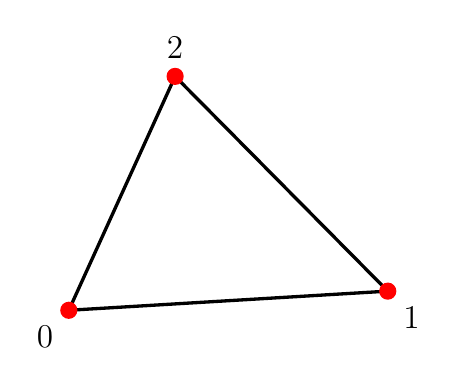
\begin{tikzpicture}[scale=1.35]
    \coordinate (A) at (0,0);
    \coordinate (B) at (3.0,0.18);
    \coordinate (C) at (1.0,2.20);

    % 三角形
    \draw[black,line width=1.2pt]
        (A)--(B)--(C)--cycle;

    % 顶点：只画红点
    \fill[red,fill opacity=1] (A) circle (2.3pt);
    \fill[red,fill opacity=1] (B) circle (2.3pt);
    \fill[red,fill opacity=1] (C) circle (2.3pt);

    % 顶点旁边直接标局部编号
    \node[
        text=black,
        font=\bfseries\large,
        below left=3pt
    ] at (A) {$0$};

    \node[
        text=black,
        font=\bfseries\large,
        below right=3pt
    ] at (B) {$1$};

    \node[
        text=black,
        font=\bfseries\large,
        above=3pt
    ] at (C) {$2$};
\end{tikzpicture}

\vspace{0.6em}

{\normalsize 三角形及其局部编号}
    \end{columns}
\end{frame}

\begin{frame}{四面体单元及其子单形}
    \begin{columns}[c]
        \column{0.55\textwidth}
        一个四面体单元 $K=[z_0,z_1,z_2,z_3]$ 包含 $4$ 个顶点、$6$ 条边、$4$ 个面和 $1$ 个三维单元。

        \vspace{1em}
        {\large
        \[
        \begin{aligned}
          \texttt{localnode} &= \{[0],[1],[2],[3]\},\\[0.4em]
          \texttt{localedge} &= \{[0,1],[0,2],[0,3],[1,2],[1,3],[2,3]\},\\[0.4em]
          \texttt{localface} &= \{[1,2,3],[0,3,2],[0,1,3],[0,2,1]\},\\[0.4em]
          \texttt{localcell} &= \{[0,1,2,3]\}.
        \end{aligned}
        \]
        }

        \column{0.45\textwidth}
        \centering
        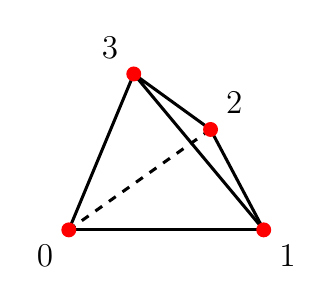
\begin{tikzpicture}[scale=1.50]
          % 与第一页的四面体保持同一投影，仅按比例缩放。
          \coordinate (A) at (2.95,-1.00);
          \coordinate (B) at (4.60,-1.00);
          \coordinate (C) at (4.15,-0.15);
          \coordinate (D) at (3.50,0.32);
          \draw[black,line width=1.1pt] (A)--(B);
          \draw[black,line width=1.1pt] (B)--(C);
          \draw[black,dashed,line width=1.1pt] (C)--(A);
          \draw[black,line width=1.1pt] (D)--(A) (D)--(B) (D)--(C);
          \foreach \P in {A,B,C,D}{\fill[red,fill opacity=1] (\P) circle (1.8pt);}
          \node[font=\bfseries\large,below left=3pt] at (A) {$0$};
          \node[font=\bfseries\large,below right=3pt] at (B) {$1$};
          \node[font=\bfseries\large,above right=3pt] at (C) {$2$};
          \node[font=\bfseries\large,above left=3pt] at (D) {$3$};
        \end{tikzpicture}

        \vspace{0.6em}
        {\normalsize 四面体及其局部编号}
    \end{columns}
\end{frame}

\begin{frame}{从单元到网格}
\begin{columns}[c]

\column{0.54\textwidth}

一个网格则由多个单元沿公共边或公共面拼接而成：

$$
\mathcal T_h=\{K_0,K_1,\ldots,K_{N_T-1}\}.
$$

\vspace{0.5em}

在程序中，网格需要同时保存：

\begin{itemize}
  \item \textbf{几何信息：}
  \texttt{node} 保存所有顶点的坐标；
  \item \textbf{拓扑信息：}
  \texttt{cell} 保存每个单元所包含的全局顶点编号。
\end{itemize}

\vspace{0.5em}

边、面以及单元之间的邻接关系，
都可以由 \texttt{cell} 进一步构造。

\column{0.46\textwidth}

\centering
\begin{tikzpicture}[scale=1.35]
  \coordinate (P0) at (0,0);
  \coordinate (P1) at (2.2,0);
  \coordinate (P2) at (2.2,2.0);
  \coordinate (P3) at (0,2.0);

  % 两个三角形
  \draw[black,line width=1.2pt]
    (P0)--(P1)--(P2)--(P3)--cycle;
  \draw[black,line width=1.2pt]
    (P0)--(P2);

  % 顶点
  \foreach \P in {P0,P1,P2,P3}{
    \fill[red] (\P) circle (2.2pt);
  }

  % 全局顶点编号
  \node[font=\bfseries\large,below left=3pt]  at (P0) {$0$};
  \node[font=\bfseries\large,below right=3pt] at (P1) {$1$};
  \node[font=\bfseries\large,above right=3pt] at (P2) {$2$};
  \node[font=\bfseries\large,above left=3pt]  at (P3) {$3$};

  % 单元编号
  \node[font=\large] at (1.48,0.58) {$K_0$};
  \node[font=\large] at (0.70,1.42) {$K_1$};

  % 公共边
  \node[
    text=blue!70!black,
    font=\small\bfseries,
    rotate=42
  ] at (1.05,1.15) {公共边};
\end{tikzpicture}

\vspace{0.6em}

{\normalsize
$$
K_0=[0,1,2],
\qquad
K_1=[0,2,3].
$$
}

\end{columns}
\end{frame}

%------------------------------------------------
\begin{frame}{三角形网格}
\begin{block}{基本数组}
\begin{itemize}
  \item \texttt{node}：大小为 $N\times 2$，第 $i$ 行是第 $i$ 个顶点的坐标；
  \item \texttt{cell}：大小为 $N_T\times 3$，第 $K$ 行给出第 $K$ 个三角形的三个顶点编号。
\end{itemize}
\end{block}

\begin{block}{辅助数据}
\begin{itemize}
  \item \texttt{edge}：大小为 $N_E\times 2$，每条边的两个端点；
  \item \texttt{cell2edge}：大小为 $N_T\times 3$，每个单元对应哪三条边；
  \item \texttt{edge2cell}：每条边邻接哪一个或两个单元；
  \item \texttt{bdFlag}：边界边标记或边界顶点标记；
  \item \texttt{elemSign} 或方向信息：记录局部边方向与全局边方向是否一致。
\end{itemize}
\end{block}

\end{frame}


\begin{frame}{三角形网格的数据结构示例}
\begin{columns}[c,onlytextwidth]

%================================================
\column{0.36\textwidth}

\centering
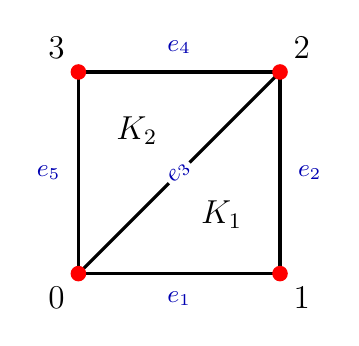
\begin{tikzpicture}[scale=1.28]
  \coordinate (P1) at (0,0);
  \coordinate (P2) at (2,0);
  \coordinate (P3) at (2,2);
  \coordinate (P4) at (0,2);

  % 网格
  \draw[black,line width=1.15pt]
    (P1)--(P2)--(P3)--(P4)--cycle;
  \draw[black,line width=1.15pt]
    (P1)--(P3);

  % 顶点
  \foreach \P in {P1,P2,P3,P4}{
    \fill[red] (\P) circle (2.2pt);
  }

  % 顶点编号
  \node[font=\bfseries\large,below left=2pt]
    at (P1) {$0$};
  \node[font=\bfseries\large,below right=2pt]
    at (P2) {$1$};
  \node[font=\bfseries\large,above right=2pt]
    at (P3) {$2$};
  \node[font=\bfseries\large,above left=2pt]
    at (P4) {$3$};

  % 单元编号
  \node[font=\large] at (1.42,0.58) {$K_1$};
  \node[font=\large] at (0.58,1.42) {$K_2$};

  % 全局边编号
  \node[
    font=\small,
    text=blue!70!black,
    below=3pt
  ] at ($(P1)!0.5!(P2)$) {$e_1$};

  \node[
    font=\small,
    text=blue!70!black,
    right=3pt
  ] at ($(P2)!0.5!(P3)$) {$e_2$};

  \node[
    font=\small,
    text=blue!70!black,
    fill=white,
    inner sep=1pt,
    rotate=45
  ] at ($(P1)!0.5!(P3)$) {$e_3$};

  \node[
    font=\small,
    text=blue!70!black,
    above=3pt
  ] at ($(P3)!0.5!(P4)$) {$e_4$};

  \node[
    font=\small,
    text=blue!70!black,
    left=3pt
  ] at ($(P4)!0.5!(P1)$) {$e_5$};
\end{tikzpicture}


%================================================
\column{0.62\textwidth}

\centering
\renewcommand{\arraystretch}{1.05}
\setlength{\abovedisplayskip}{2pt}
\setlength{\belowdisplayskip}{2pt}

% 第一列：node / cell
\begin{minipage}[t]{0.27\linewidth}
\vspace{0pt}
\centering

\begin{minipage}[t][3.35cm][t]{\linewidth}
\centering
{\large\bfseries\texttt{node}}

$$
\begin{bmatrix}
0&0\\
2&0\\
2&2\\
0&2
\end{bmatrix}
$$
\end{minipage}
\vspace{0.8em}

{\large\bfseries\texttt{cell}}

$$
\begin{bmatrix}
0&1&2\\
0&2&3
\end{bmatrix}
$$

\end{minipage}
\hfill
% 第二列：edge / cell2edge
\begin{minipage}[t]{0.32\linewidth}
\vspace{0pt}
\centering

\begin{minipage}[t][3.35cm][t]{\linewidth}
\centering
{\large\bfseries\texttt{edge}}

$$
\begin{bmatrix}
0&1\\
1&2\\
0&2\\
2&3\\
0&3
\end{bmatrix}
$$
\end{minipage}
\vspace{0.8em}

{\large\bfseries\texttt{cell2edge}}

$$
\begin{bmatrix}
0&1&2\\
2&3&4
\end{bmatrix}
$$

\end{minipage}
\hfill
% 第三列：edge2cell / bdEdgeFlag
\begin{minipage}[t]{0.35\linewidth}
\vspace{0pt}
\centering

\begin{minipage}[t][3.35cm][t]{\linewidth}
\centering
{\large\bfseries\texttt{edge2cell}}

$$
\begin{bmatrix}
0&0\\
0&0\\
0&1\\
1&1\\
1&1
\end{bmatrix}
$$
\end{minipage}
\vspace{0.8em}

{\large\bfseries\texttt{bdEdgeFlag}}

$$
\begin{bmatrix}
1&1&0&1&1
\end{bmatrix}
$$

\end{minipage}

\end{columns}
\end{frame}


%------------------------------------------------
\begin{frame}{四面体网格}

\begin{block}{基本数组}
\begin{itemize}
  \item \texttt{node}：大小为 $N\times 3$，第 $i$ 行是第 $i$ 个顶点的坐标；
  \item \texttt{cell}：大小为 $N_T\times 4$，第 $K$ 行给出第 $K$ 个四面体的四个顶点编号。
\end{itemize}
\end{block}

\begin{block}{辅助数据}
\begin{itemize}
  \item \texttt{edge}：大小为 $N_E\times 2$，每条边的两个端点；
  \item \texttt{face}：大小为 $N_F\times 3$，每个面的三个顶点；
  \item \texttt{cell2edge}：大小为 $N_T\times 6$，每个单元对应的六条边；
  \item \texttt{cell2face}：大小为 $N_T\times 4$，每个单元对应的四个面；
  \item \texttt{face2cell}：每个面邻接的一个或两个单元；
  \item \texttt{bdFaceFlag}：标记每个面是否为边界面；
  \item \texttt{faceSign}：记录局部面方向与全局面方向是否一致。
\end{itemize}
\end{block}

\end{frame}


%------------------------------------------------
\begin{frame}{四面体网格的数据结构示例}
\begin{columns}[c,onlytextwidth]

%================================================
\column{0.30\textwidth}

\centering
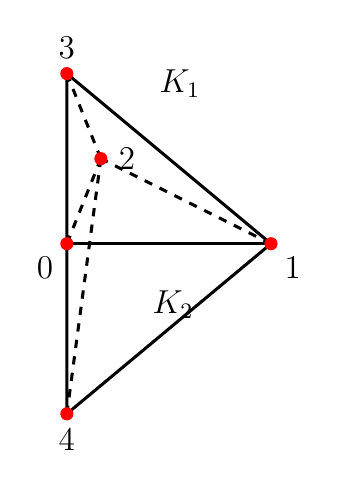
\begin{tikzpicture}[scale=1.08]
  % 公共面的三个顶点
  \coordinate (P1) at (0,0);
  \coordinate (P2) at (2.4,0);
  \coordinate (P3) at (0.4,1.0);

  % 两个四面体的顶点
  \coordinate (P4) at (0,2);
  \coordinate (P5) at (0,-2);

  % 与原编号 3（现编号 2）相连的边为隐藏边，画成虚线。
  \draw[black,line width=1.1pt] (P1)--(P2);
  \draw[black,dashed,line width=1.1pt] (P2)--(P3) (P3)--(P1);

  % 上侧四面体 K_1
  \draw[black,line width=1.1pt] (P4)--(P1) (P4)--(P2);
  \draw[black,dashed,line width=1.1pt] (P4)--(P3);

  % 下侧四面体 K_2
  \draw[black,line width=1.1pt] (P5)--(P1) (P5)--(P2);
  \draw[black,dashed,line width=1.1pt] (P5)--(P3);

  % 顶点
  \foreach \P in {P1,P2,P3,P4,P5}{
    \fill[red] (\P) circle (2.2pt);
  }

  % 顶点编号
  \node[font=\bfseries\large,below left=2pt]
    at (P1) {$0$};

  \node[font=\bfseries\large,below right=2pt]
    at (P2) {$1$};

  \node[font=\bfseries\large,right=3pt]
    at (P3) {$2$};

  \node[font=\bfseries\large,above=2pt]
    at (P4) {$3$};

  \node[font=\bfseries\large,below=2pt]
    at (P5) {$4$};

  % 单元编号
  \node[font=\large] at (1.33,1.88) {$K_1$};
  \node[font=\large] at (1.25,-0.72) {$K_2$};

\end{tikzpicture}


%================================================
\column{0.68\textwidth}

\centering
\renewcommand{\arraystretch}{1.02}
\setlength{\abovedisplayskip}{2pt}
\setlength{\belowdisplayskip}{2pt}

{\small

%------------------------------------------------
% 第一列：node / cell
\begin{minipage}[t]{0.22\linewidth}
\vspace{0pt}
\centering

\begin{minipage}[t][3.75cm][t]{\linewidth}
\centering
{\normalsize\bfseries\texttt{node}}

$$
\begin{bmatrix}
0&0&0\\
2&0&0\\
0&2&0\\
0&0&2\\
0&0&-2
\end{bmatrix}
$$
\end{minipage}

\iffalse

\vspace{0.5em}

{\normalsize\bfseries\texttt{cell}}

$$
\begin{bmatrix}
0&1&2&3\\
0&2&1&4
\end{bmatrix}
$$

\end{minipage}
\fi
\end{minipage}
\hfill
%------------------------------------------------
% 第二列：edge / cell2edge
\begin{minipage}[t]{0.23\linewidth}
\vspace{0pt}
\centering

\begin{minipage}[t][3.75cm][t]{\linewidth}
\centering
{\normalsize\bfseries\texttt{edge}}

$$
\begin{bmatrix}
0&1\\
0&2\\
1&2\\
0&3\\
1&3\\
2&3\\
0&4\\
1&4\\
2&4
\end{bmatrix}
$$
\end{minipage}

\iffalse

\vspace{0.5em}

{\normalsize\bfseries\texttt{cell2edge}}

$$
\begin{bmatrix}
0&1&2&3&4&5\\
0&1&2&6&7&8
\end{bmatrix}
$$

\end{minipage}
\fi
\end{minipage}
\hfill
%------------------------------------------------
% 第三列：face / cell2face
\begin{minipage}[t]{0.26\linewidth}
\vspace{0pt}
\centering

\begin{minipage}[t][3.75cm][t]{\linewidth}
\centering
{\normalsize\bfseries\texttt{face}}

$$
\begin{bmatrix}
0&1&2\\
0&1&3\\
0&2&3\\
1&2&3\\
0&1&4\\
0&2&4\\
1&2&4
\end{bmatrix}
$$
\end{minipage}

\iffalse

\vspace{0.5em}

{\normalsize\bfseries\texttt{cell2face}}

$$
\begin{bmatrix}
0&1&2&3\\
0&4&5&6
\end{bmatrix}
$$

\end{minipage}
\fi
\end{minipage}
\hfill
%------------------------------------------------
% 第四列：face2cell / bdFaceFlag
\begin{minipage}[t]{0.25\linewidth}
\vspace{0pt}
\centering

\begin{minipage}[t][3.75cm][t]{\linewidth}
\centering
{\normalsize\bfseries\texttt{face2cell}}

$$
\begin{bmatrix}
0&1\\
0&0\\
0&0\\
0&0\\
1&1\\
1&1\\
1&1
\end{bmatrix}
$$
\end{minipage}

\iffalse

\vspace{0.5em}

{\normalsize\bfseries\texttt{bdFaceFlag}}

$$
\begin{bmatrix}
0&1&1&1&1&1&1
\end{bmatrix}
$$

\end{minipage}
\fi
\end{minipage}

}

\end{columns}
\end{frame}

%------------------------------------------------
\begin{frame}{四面体网格的数据结构示例（续）}
\begin{columns}[c,onlytextwidth]
\column{0.30\textwidth}
\centering
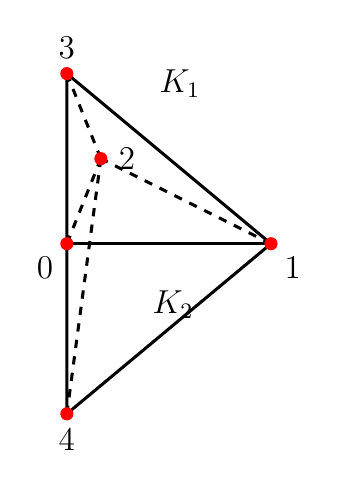
\begin{tikzpicture}[scale=1.08]
  \coordinate (P1) at (0,0); \coordinate (P2) at (2.4,0);
  \coordinate (P3) at (0.4,1.0); \coordinate (P4) at (0,2);
  \coordinate (P5) at (0,-2);
  \draw[black,line width=1.1pt] (P1)--(P2);
  \draw[black,dashed,line width=1.1pt] (P2)--(P3) (P3)--(P1);
  \draw[black,line width=1.1pt] (P4)--(P1) (P4)--(P2);
  \draw[black,dashed,line width=1.1pt] (P4)--(P3);
  \draw[black,line width=1.1pt] (P5)--(P1) (P5)--(P2);
  \draw[black,dashed,line width=1.1pt] (P5)--(P3);
  \foreach \P in {P1,P2,P3,P4,P5}{\fill[red] (\P) circle (2.2pt);}
  \node[font=\bfseries\large,below left=2pt] at (P1) {$0$};
  \node[font=\bfseries\large,below right=2pt] at (P2) {$1$};
  \node[font=\bfseries\large,right=3pt] at (P3) {$2$};
  \node[font=\bfseries\large,above=2pt] at (P4) {$3$};
  \node[font=\bfseries\large,below=2pt] at (P5) {$4$};
  \node[font=\large] at (1.33,1.88) {$K_1$};
  \node[font=\large] at (1.25,-0.72) {$K_2$};
\end{tikzpicture}

\column{0.68\textwidth}
\centering
\renewcommand{\arraystretch}{1.15}
\begin{columns}[c,onlytextwidth]
\column{0.46\textwidth}\centering
{\large\bfseries\texttt{cell}}
\[\begin{bmatrix}0&1&2&3\\0&2&1&4\end{bmatrix}\]
\column{0.46\textwidth}\centering
{\large\bfseries\texttt{cell2edge}}
\[\begin{bmatrix}0&1&2&3&4&5\\0&1&2&6&7&8\end{bmatrix}\]
\end{columns}

\vspace{1.2em}
\begin{columns}[c,onlytextwidth]
\column{0.46\textwidth}\centering
{\large\bfseries\texttt{cell2face}}
\[\begin{bmatrix}0&1&2&3\\0&4&5&6\end{bmatrix}\]
\column{0.46\textwidth}\centering
{\large\bfseries\texttt{bdFaceFlag}}
\[\begin{bmatrix}0&1&1&1&1&1&1\end{bmatrix}\]
\end{columns}
\end{columns}
\end{frame}

%================================================
\section{Hu-Zhang 基函数}

\begin{frame}{重心坐标函数}

设单纯形
$
K=[z_0,z_1, \cdots, z_d],
$
定义 $d+1$ 个线性函数 $\lambda_i : K -> \mathbb{R}$，满足：
$$
\lambda_i(z_j) = \delta_{ij}, \sum_{\lambda_i} = 1.
$$

那么对任意 $x\in K$，
$
x = \sum_{i=0}^{d}\lambda_i(x)z_i.
$

\vspace{0.5em}
\begin{center}
  \includegraphics[width=0.88\textwidth]{figures/barycentric_coordinates.png}
\end{center}

\end{frame}

%------------------------------------------------
\begin{frame}{单纯形上的等距格点}
\begin{columns}[c,onlytextwidth]

\column{0.6\textwidth}

对给定次数 $k$，定义多重指标集合
$$
\mathbb T_d^k
=
\left\{
\alpha=(\alpha_0,\ldots,\alpha_d)\in\mathbb N_0^{d+1}
:
|\alpha|=\sum_{i=0}^{d}\alpha_i=k
\right\}.
$$

与 $\alpha\in\mathbb T_d^k$ 对应的等距格点为
$$
x_\alpha
=
\sum_{i=0}^{d}\frac{\alpha_i}{k}z_i,
\qquad
\lambda_i(x_\alpha)=\frac{\alpha_i}{k}.
$$

记
\(
f_\alpha=[z_i:\alpha_i>0]
\)，即由 $\alpha$ 的非零分量对应顶点张成的最大子单形。
格点总数为
$$
\#\mathbb T_d^k
=
\binom{k+d}{d}
=
\dim\mathbb P_k(K).
$$

\column{0.39\textwidth}

\centering
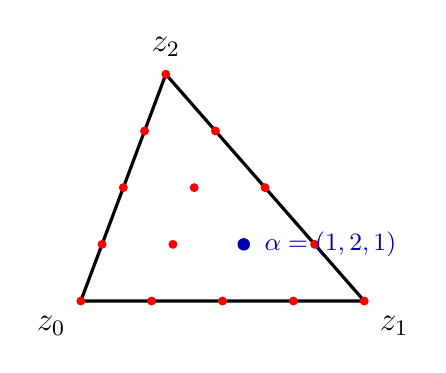
\begin{tikzpicture}[scale=0.9]
  \coordinate (A) at (0,0);
  \coordinate (B) at (4,0);
  \coordinate (C) at (1.2,3.2);

  \draw[black,line width=1.15pt]
    (A)--(B)--(C)--cycle;

  % k=4 等距格点
  \foreach \i in {0,...,4}{
    \pgfmathtruncatemacro{\m}{4-\i}
    \foreach \j in {0,...,\m}{
      \pgfmathsetmacro{\px}{(\i*4.0+\j*1.2)/4}
      \pgfmathsetmacro{\py}{(\j*3.2)/4}
      \fill[red] (\px,\py) circle (1.8pt);
    }
  }

  % 顶点编号
  \node[font=\bfseries\large,below left=3pt]
    at (A) {$z_0$};

  \node[font=\bfseries\large,below right=3pt]
    at (B) {$z_1$};

  \node[font=\bfseries\large,above=3pt]
    at (C) {$z_2$};

  % 选中的格点 alpha=(1,2,1)
  \fill[blue!70!black] (2.3,0.8) circle (2.5pt);

  \node[
    text=blue!70!black,
    font=\small\bfseries,
    right=4pt
  ] at (2.3,0.8) {$\alpha=(1,2,1)$};
\end{tikzpicture}

\vspace{0.6em}

{\normalsize 三角形上的 $4$ 次等距格点}
\vspace{2em}

\end{columns}
\end{frame}


%------------------------------------------------
\begin{frame}{Lagrange 插值基函数}

对每个 $\alpha\in\mathbb T_d^k$，定义
$$
\ell_m^{(k)}(t)
=
\frac{1}{m!}
\prod_{j=0}^{m-1}(kt-j),
\qquad
\ell_0^{(k)}(t)=1.
$$

对应的 Lagrange 基函数为
$$
\phi_\alpha(x)
=
\prod_{i=0}^{d}
\ell_{\alpha_i}^{(k)}\bigl(\lambda_i(x)\bigr)
=
\frac{1}{\alpha_0!\cdots\alpha_d!}
\prod_{i=0}^{d}
\prod_{j=0}^{\alpha_i-1}
\bigl(k\lambda_i(x)-j\bigr).
$$

它满足节点插值性质
$$
\phi_\alpha(x_\beta)
=
\delta_{\alpha\beta},
\qquad
\alpha,\beta\in\mathbb T_d^k.
$$
\vspace{0.01em}

因此
$
\mathbb P_k(K)
=
\operatorname{span}
\left\{
\phi_\alpha:\alpha\in\mathbb T_d^k
\right\}.
$

\end{frame}

%------------------------------------------------
\begin{frame}{三角形上三次 Lagrange 元}
\begin{columns}[c,onlytextwidth]

\column{0.43\textwidth}

\centering
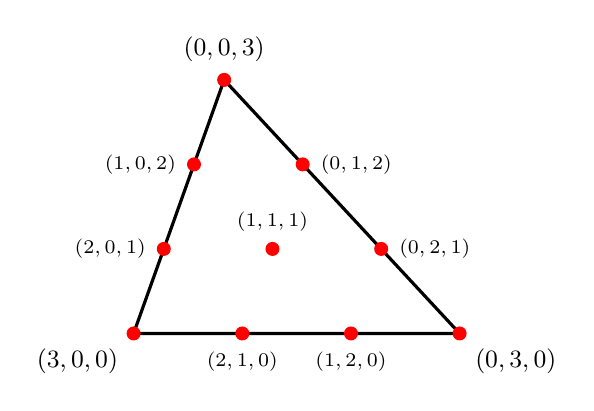
\begin{tikzpicture}[scale=1.15]
  \coordinate (A) at (0,0);
  \coordinate (B) at (3.6,0);
  \coordinate (C) at (1.0,2.8);
  \coordinate (P01) at ($(A)!1/3!(B)$);
  \coordinate (P02) at ($(A)!2/3!(B)$);
  \coordinate (P12) at ($(B)!1/3!(C)$);
  \coordinate (P21) at ($(B)!2/3!(C)$);
  \coordinate (P20) at ($(C)!1/3!(A)$);
  \coordinate (P10) at ($(C)!2/3!(A)$);
  \coordinate (G) at (1.5333,0.9333);

  \draw[black,line width=1.15pt]
    (A)--(B)--(C)--cycle;

  \foreach \P in {A,B,C,P01,P02,P12,P21,P20,P10,G}{
    \fill[red] (\P) circle (2.2pt);
  }

  \node[font=\small\bfseries,below left=3pt]
    at (A) {$(3,0,0)$};

  \node[font=\small\bfseries,below right=3pt]
    at (B) {$(0,3,0)$};

  \node[font=\small\bfseries,above=3pt]
    at (C) {$(0,0,3)$};

  \node[font=\scriptsize,below=3pt] at (P01) {$(2,1,0)$};
  \node[font=\scriptsize,below=3pt] at (P02) {$(1,2,0)$};
  \node[font=\scriptsize,right=3pt] at (P12) {$(0,2,1)$};
  \node[font=\scriptsize,right=3pt] at (P21) {$(0,1,2)$};
  \node[font=\scriptsize,left=3pt] at (P20) {$(1,0,2)$};
  \node[font=\scriptsize,left=3pt] at (P10) {$(2,0,1)$};
  \node[font=\scriptsize,above=3pt] at (G) {$(1,1,1)$};
\end{tikzpicture}

\vspace{0.7em}

{\normalsize $10$ 个格点对应 $10$ 个局部自由度}

\column{0.55\textwidth}

对 $k=3$，顶点基函数为
$$
\begin{aligned}
\phi_{300}&=\tfrac12\lambda_0(3\lambda_0-1)(3\lambda_0-2),\\
\phi_{030}&=\tfrac12\lambda_1(3\lambda_1-1)(3\lambda_1-2),\\
\phi_{003}&=\tfrac12\lambda_2(3\lambda_2-1)(3\lambda_2-2).
\end{aligned}
$$

例如边 $[z_0,z_1]$ 上的两个基函数为
$$
\begin{aligned}
\phi_{210}&=\tfrac92\lambda_0\lambda_1(3\lambda_0-1),\\
\phi_{120}&=\tfrac92\lambda_0\lambda_1(3\lambda_1-1),\\
\phi_{111}&=27\lambda_0\lambda_1\lambda_2.
\end{aligned}
$$

\end{columns}
\end{frame}

\begin{frame}{三角形上的三次 Lagrange 节点基函数}
令 $p=3$。三角形上共有 $\binom{p+2}{2}=10$ 个等距格点；下面给出顶点、边与内部的典型节点基函数图像。

\vspace{0.2em}
\begin{center}
  \includegraphics[width=0.96\textwidth]{figures/lagrange_p3_basis.pdf}
\end{center}

\vspace{-0.4em}
\end{frame}

\begin{frame}
    \frametitle{局部基函数的"拼接"（边）}
    对共享边，两个单元上的三次局部基函数只要在该边上的迹相同，就可以拼接成一个全局连续函数。

    \vspace{0.3em}
    \begin{center}
      \includegraphics[height=0.8\textheight,keepaspectratio]{figures/lagrange_gluing_edge.pdf}
    \end{center}

\end{frame}

\begin{frame}
    \frametitle{局部基函数的"拼接"（节点）}
    对共享顶点，围绕该点的三次局部顶点基函数可以拼为一个全局节点基函数。

    \vspace{0.3em}
    \begin{center}
        \includegraphics[height=0.8\textheight,keepaspectratio]{figures/lagrange_gluing_node.pdf}
    \end{center}

\end{frame}

\begin{frame}
  \frametitle{$\mathbb{S}$ 的分解}

\begin{columns}[c,onlytextwidth]
\column{0.6\textwidth}
设 $f\in\Delta_\ell(K)$，取切向基 $\{t_{f,i}\}_{i=0}^{\ell-1}$ 与法向基
$\{n_{f,j}\}_{j=0}^{d-\ell-1}$。
\[
\begin{aligned}
\mathcal T^f(\mathbb S)
&=\operatorname{span}\!\left\{
\operatorname{sym}(t_{f,i}\otimes t_{f,j})\right\},\\
\mathcal N^f(\mathbb S)
&=\operatorname{span}\!\left\{
\operatorname{sym}(n_{f,i}\otimes n_{f,j}),\
\operatorname{sym}(t_{f,i}\otimes n_{f,j})\right\}.
\end{aligned}
\]
\[
\boxed{\quad
\mathbb S=\mathcal T^f(\mathbb S)\oplus\mathcal N^f(\mathbb S)\quad}
\]

\small
\(\mathcal T^f(\mathbb S)\) 是纯切向部分，满足 $\tau n_f=0$，可在 $f$ 上断开；
\(\mathcal N^f(\mathbb S)\) 含法向分量，负责跨 $f$ 的连续性。

\column{0.4\textwidth}
\centering
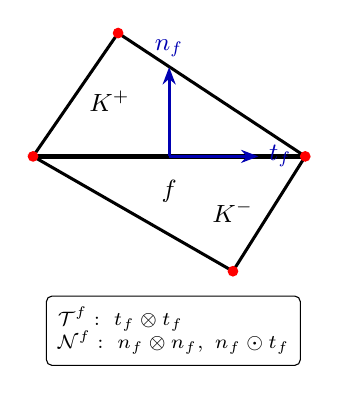
\begin{tikzpicture}[scale=1.08]
  \coordinate (A) at (0,0);
  \coordinate (B) at (3.2,0);
  \coordinate (U) at (1.0,1.45);
  \coordinate (D) at (2.35,-1.35);
  \coordinate (M) at (1.6,0);
  \draw[black,line width=1.1pt] (A)--(B)--(U)--cycle;
  \draw[black,line width=1.1pt] (A)--(B)--(D)--cycle;
  \draw[black,line width=1.7pt] (A)--(B);
  \foreach \P in {A,B,U,D}{\fill[red] (\P) circle (1.8pt);}
  \draw[-{Stealth[length=2.2mm]},blue!70!black,line width=1.1pt] (M)--++(1.05,0) node[right] {$t_f$};
  \draw[-{Stealth[length=2.2mm]},blue!70!black,line width=1.1pt] (M)--++(0,1.05) node[above] {$n_f$};
  \node[below=5pt] at (M) {$f$};
  \node[font=\small] at (0.9,0.65) {$K^+$};
  \node[font=\small] at (2.35,-0.65) {$K^-$};
  \node[align=left,font=\scriptsize,draw=black,rounded corners=2pt,inner sep=4pt] at (1.65,-2.05)
    {$\mathcal T^f:\ t_f\otimes t_f$\\[-1pt]$\mathcal N^f:\ n_f\otimes n_f,\ n_f\odot t_f$};
\end{tikzpicture}
\end{columns}

\end{frame}

%------------------------------------------------
\begin{frame}{$\mathbb{S}$ 的分解}
\begin{columns}[c,onlytextwidth]
\column{0.50\textwidth}
\centering
\includegraphics[width=\textwidth,height=0.80\textheight,keepaspectratio]{figures/HuZhangFrame.pdf}

\column{0.50\textwidth}
\centering
\includegraphics[width=\textwidth,height=0.80\textheight,keepaspectratio]{figures/frame3d.pdf}
\end{columns}
\end{frame}

\begin{frame}{Hu--Zhang 元的局部自由度}
\begin{columns}[c,onlytextwidth]
\column{0.54\textwidth}


对每个格点 $\alpha\in\mathbb T_d^k$，令 $f=f_\alpha$。
任意 $$\boldsymbol{\sigma} \in \mathbb{P}_k(T; \mathbb{S})$$都可以由如下自由度唯一决定：
$$
\begin{aligned}
\boldsymbol{\sigma}(\boldsymbol{x}_{\boldsymbol{\alpha}}) : \boldsymbol{N}  \quad
\boldsymbol{\alpha} \in \mathbb{T}_k^d, \boldsymbol{N} \in
\mathcal{ N}_f(\mathbb{S}), \qquad (1)\\
\boldsymbol{\sigma}(\boldsymbol{x}_{\boldsymbol{\alpha}}) : \boldsymbol{T}
\quad \boldsymbol{\alpha} \in \mathbb{T}_k^d, \boldsymbol{T} \in
\mathcal{ T}_f(\mathbb{S}). \qquad (2)
\end{aligned}
$$
其中 $:$ 表示 Frobenius 内积。

单纯形网格 $\mathcal{T}_h$ 上的 Hu-Zhang 元空间为：
$$\begin{aligned}
\Sigma_h^k := \{\boldsymbol{\sigma} \in L^2(\Omega, \mathbb{S})\ :\ \
    &\boldsymbol{\sigma}|_T \in \mathbb{P}_k(T, \mathbb{S}), \forall T \in
    \mathcal{T}_h;\\
    &\text{ 且 } \forall f \in \Delta \mathcal{T}_h, \text{自由度 (1)
    在 $f$ 上是单值的。} \}
\end{aligned}$$

\column{0.42\textwidth}
\centering
\includegraphics[width=\textwidth,height=0.76\textheight,keepaspectratio]{figures/HuZhangFrame.pdf}
\end{columns}

\end{frame}

\begin{frame}{Hu--Zhang 元的局部基函数}
\begin{columns}[c,onlytextwidth]
\column{0.54\textwidth}
\small

设 $\phi_\alpha$ 是格点 $x_\alpha$ 对应的 Lagrange 基函数。
根据 Lagrange 元基函数的对偶性以及标架的正交性，以上自由度的基函数可以显式写出：
$$
\begin{aligned}
\boldsymbol{\phi}_{\boldsymbol{\alpha}}\otimes \boldsymbol{N} \quad &
\boldsymbol{\alpha} \in \mathbb{T}_k^d,\ \boldsymbol{N} \in
\mathcal{N}_f(\mathbb{S}), \\
\boldsymbol{\phi}_{\boldsymbol{\alpha}}\otimes \boldsymbol{T} \quad &
\boldsymbol{\alpha} \in \mathbb{T}_k^d,\ \boldsymbol{T} \in
\mathcal{T}_f(\mathbb{S}).
\end{aligned}
$$

\column{0.42\textwidth}
\centering
\includegraphics[width=\textwidth,height=0.76\textheight,keepaspectratio]{figures/HuZhangFrame.pdf}
\end{columns}

\end{frame}


\begin{frame}{二维 $\mathbb P_3$ Hu--Zhang 元的局部基函数（顶点）}
\begin{columns}[c,onlytextwidth]

\column{0.42\textwidth}
\centering
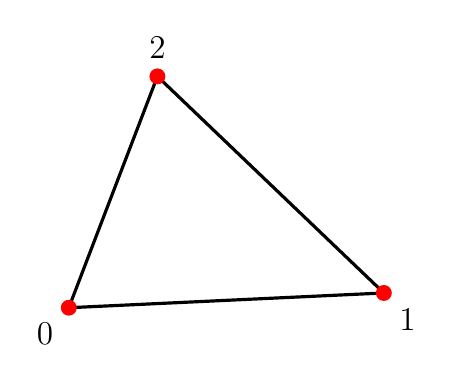
\begin{tikzpicture}[scale=1.25]
  \coordinate (A) at (0,0);
  \coordinate (B) at (3.2,0.15);
  \coordinate (C) at (0.9,2.35);
  \draw[black,line width=1.15pt] (A)--(B)--(C)--cycle;
  \foreach \P/\lab in {A/0,B/1,C/2}{
    \fill[red] (\P) circle (2.3pt);
  }
  \node[font=\bfseries\large,below left=3pt] at (A) {$0$};
  \node[font=\bfseries\large,below right=3pt] at (B) {$1$};
  \node[font=\bfseries\large,above=3pt] at (C) {$2$};
\end{tikzpicture}

\column{0.56\textwidth}

三个顶点基函数为：
$$
\begin{aligned}
\phi_{300}=\tfrac12\lambda_0(3\lambda_0-1)(3\lambda_0-2),\\
\phi_{030}=\tfrac12\lambda_1(3\lambda_1-1)(3\lambda_1-2),\\
\phi_{003}=\tfrac12\lambda_2(3\lambda_2-1)(3\lambda_2-2),\\
\end{aligned}
$$

二维对称矩阵空间取基
$$
E_1=
\begin{bmatrix}1&0\\0&0\end{bmatrix},
\quad
E_2=
\begin{bmatrix}0&1\\1&0\end{bmatrix},
\quad
E_3=
\begin{bmatrix}0&0\\0&1\end{bmatrix}.
$$

每个顶点给出 $3$ 个矩阵值基函数：
$$
\phi_{300} E_i,
\qquad
\phi_{030} E_i,
\qquad
\phi_{003} E_i,
\qquad i=0,1,2.
$$

\end{columns}
\end{frame}

\begin{frame}{二维 $\mathbb P_3$ Hu--Zhang 元的局部基函数（边）}
\begin{columns}[c,onlytextwidth]

\column{0.42\textwidth}
\centering
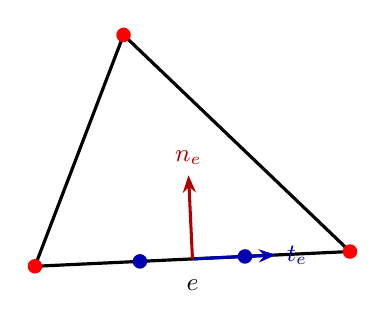
\begin{tikzpicture}[scale=1.25]
  \coordinate (A) at (0,0);
  \coordinate (B) at (3.2,0.15);
  \coordinate (C) at (0.9,2.35);
  \draw[black,line width=1.15pt] (A)--(B)--(C)--cycle;
  \foreach \P in {A,B,C}{\fill[red] (\P) circle (2.1pt);}
  \fill[blue!70!black] ($(A)!1/3!(B)$) circle (2.1pt);
  \fill[blue!70!black] ($(A)!2/3!(B)$) circle (2.1pt);
  \node[below=4pt] at ($(A)!0.5!(B)$) {$e$};
  \draw[-{Stealth[length=2.2mm]},blue!70!black,line width=1.1pt]
    ($(A)!0.5!(B)$)--++(0.85,0.04) node[right] {$t_e$};
  \draw[-{Stealth[length=2.2mm]},red!70!black,line width=1.1pt]
    ($(A)!0.5!(B)$)--++(-0.04,0.85) node[above] {$n_e$};
\end{tikzpicture}

\column{0.56\textwidth}

以边 $e=[z_0,z_1]$ 为例，两个边内标量基函数为
$$
\psi_{e,1}=\phi_{210}=\tfrac92\lambda_0\lambda_1(3\lambda_0-1),
$$
$$
\psi_{e,2}=\phi_{120}=\tfrac92\lambda_0\lambda_1(3\lambda_1-1).
$$

负责跨边连续的是法向部分
$$
\mathcal N^e(\mathbb S)
=
\operatorname{span}\{n_e\otimes n_e,\operatorname{sym}(t_e\otimes n_e)\}.
$$

对应基函数为
$$
\psi_{e,r}(n_e\otimes n_e),
\quad
\psi_{e,r}\operatorname{sym}(t_e\otimes n_e),
\qquad r = 1, 2.
$$

\end{columns}
\end{frame}

\begin{frame}{二维 $\mathbb P_3$ Hu--Zhang 元的局部基函数（边 bubble）}
\begin{columns}[c,onlytextwidth]

\column{0.42\textwidth}
\centering
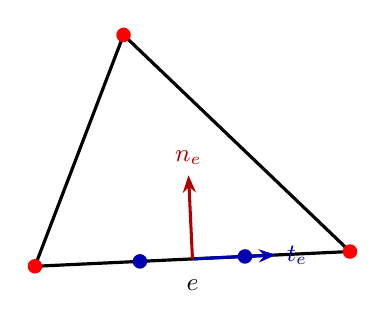
\begin{tikzpicture}[scale=1.25]
  \coordinate (A) at (0,0);
  \coordinate (B) at (3.2,0.15);
  \coordinate (C) at (0.9,2.35);
  \draw[black,line width=1.15pt] (A)--(B)--(C)--cycle;
  \foreach \P in {A,B,C}{\fill[red] (\P) circle (2.1pt);}
  \fill[blue!70!black] ($(A)!1/3!(B)$) circle (2.1pt);
  \fill[blue!70!black] ($(A)!2/3!(B)$) circle (2.1pt);
  \node[below=4pt] at ($(A)!0.5!(B)$) {$e$};
  \draw[-{Stealth[length=2.2mm]},blue!70!black,line width=1.1pt]
    ($(A)!0.5!(B)$)--++(0.85,0.04) node[right] {$t_e$};
  \draw[-{Stealth[length=2.2mm]},red!70!black,line width=1.1pt]
    ($(A)!0.5!(B)$)--++(-0.04,0.85) node[above] {$n_e$};
\end{tikzpicture}

\column{0.56\textwidth}

边上的切向向部分
$$
\mathcal T^e(\mathbb S)
=
\operatorname{span}\{t_e\otimes t_e\}.
$$
对应基函数为
$$
\psi_{e,r}(t_e\otimes t_e),
\qquad r=1,2.
$$

\end{columns}
\end{frame}

\begin{frame}{二维 $\mathbb P_3$ Hu--Zhang 元的局部基函数（内部 bubble）}
\begin{columns}[c,onlytextwidth]

\column{0.42\textwidth}
\centering
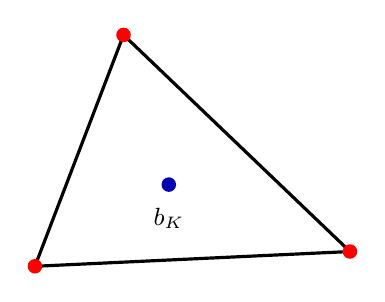
\begin{tikzpicture}[scale=1.25]
  \coordinate (A) at (0,0);
  \coordinate (B) at (3.2,0.15);
  \coordinate (C) at (0.9,2.35);
  \draw[black,line width=1.15pt] (A)--(B)--(C)--cycle;
  \foreach \P in {A,B,C}{\fill[red] (\P) circle (2.1pt);}
  \fill[blue!70!black] (1.36,0.83) circle (2.1pt);
  \node[font=\small,below=5pt] at (1.36,0.83) {$b_K$};
\end{tikzpicture}

\column{0.56\textwidth}

三角形三次元只有一个内部标量 bubble：
$$
b_K=\phi_{111}=27\lambda_0\lambda_1\lambda_2.
$$

它在整个边界上为零：
$$
b_K|_{\partial K}=0.
$$

因此内部 bubble 可以乘以任意对称矩阵方向：
$$
b_K E_1,
\qquad
b_K E_2,
\qquad
b_K E_3.
$$

\end{columns}
\end{frame}

\begin{frame}{Hu--Zhang 基函数拼接}
\begin{columns}[c,onlytextwidth]

\column{0.46\textwidth}
\centering
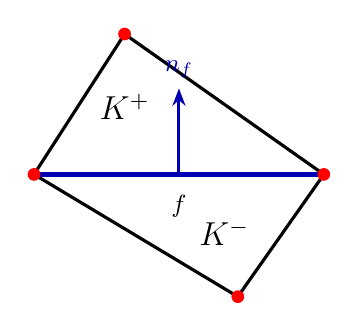
\begin{tikzpicture}[scale=1.15]
  \coordinate (A) at (0,0);
  \coordinate (B) at (3.2,0);
  \coordinate (U) at (1.0,1.55);
  \coordinate (D) at (2.25,-1.35);
  \draw[black,line width=1.15pt] (A)--(B)--(U)--cycle;
  \draw[black,line width=1.15pt] (A)--(B)--(D)--cycle;
  \draw[blue!70!black,line width=1.8pt] (A)--(B);
  \foreach \P in {A,B,U,D}{\fill[red] (\P) circle (2pt);}
  \node[font=\large] at (1.0,0.75) {$K^+$};
  \node[font=\large] at (2.1,-0.65) {$K^-$};
  \node[below=4pt] at ($(A)!0.5!(B)$) {$f$};
  \draw[-{Stealth[length=2.2mm]},blue!70!black,line width=1.1pt]
    ($(A)!0.5!(B)$)--++(0,0.95) node[above] {$n_f$};
\end{tikzpicture}

\column{0.52\textwidth}

在公共边 $f$ 上，Hu--Zhang 元要求
$$
(\tau^+ n_f)|_f=(\tau^- n_f)|_f.
$$

因此：
\begin{itemize}
  \item $\mathcal N^f(\mathbb S)$ 方向上的自由度使用同一个全局编号；
  \item $\mathcal T^f(\mathbb S)$ 方向满足 $\tau n_f=0$，不需要跨单元拼接；
  \item 单元内部 bubble 完全局部。
\end{itemize}

\vspace{0.4em}

编程核心：
$$
\texttt{elem2dof}
=
\text{共享 dof} + \text{局部 bubble dof}.
$$

\end{columns}
\end{frame}

\section{自由度管理}

\begin{frame}{局部格点编号}
\begin{columns}[c,onlytextwidth]
\column{0.34\textwidth}

局部格点按照所在子单形的维数递增编号：

\[
\text{顶点}
\;\longrightarrow\;
\text{边内点}
\;\longrightarrow\;
\text{单元内部点}.
\]

\column{0.62\textwidth}
\centering
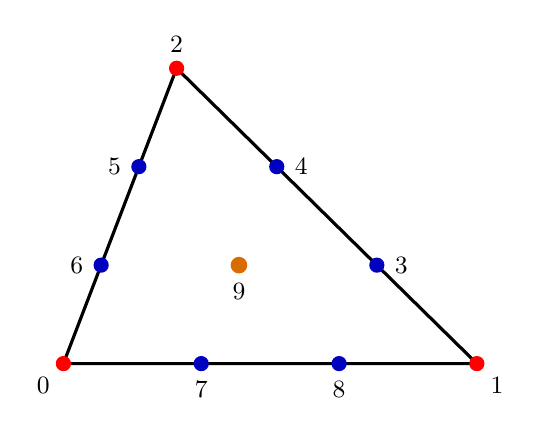
\begin{tikzpicture}[scale=1.25]
  \coordinate (A) at (0,0);
  \coordinate (B) at (4.2,0);
  \coordinate (C) at (1.15,3.0);
  \coordinate (P01) at ($(A)!1/3!(B)$);
  \coordinate (P02) at ($(A)!2/3!(B)$);
  \coordinate (P12) at ($(B)!1/3!(C)$);
  \coordinate (P21) at ($(B)!2/3!(C)$);
  \coordinate (P20) at ($(C)!1/3!(A)$);
  \coordinate (P10) at ($(C)!2/3!(A)$);
  \coordinate (G) at (1.7833,1.0);

  \draw[black,line width=1.15pt] (A)--(B)--(C)--cycle;
  \foreach \P in {A,B,C}{
    \fill[red] (\P) circle (2.2pt);
  }
  \foreach \P in {P01,P02,P12,P21,P20,P10}{
    \fill[blue!75!black] (\P) circle (2.2pt);
  }
  \fill[orange!85!black] (G) circle (2.4pt);

  \node[below left=2pt] at (A) {$0$};
  \node[below right=2pt] at (B) {$1$};
  \node[above=2pt] at (C) {$2$};
  \node[below=3pt] at (P01) {$7$};
  \node[below=3pt] at (P02) {$8$};
  \node[right=3pt] at (P12) {$3$};
  \node[right=3pt] at (P21) {$4$};
  \node[left=3pt] at (P20) {$5$};
  \node[left=3pt] at (P10) {$6$};
  \node[below=3pt] at (G) {$9$};
\end{tikzpicture}

\end{columns}
\end{frame}

\begin{frame}{全局格点编号}

全局格点编号按照网格实体生成：
$$
\texttt{node}\quad\rightarrow\quad
\texttt{edge}\quad\rightarrow\quad
\texttt{face}\quad\rightarrow\quad
\texttt{cell}.
$$

\vspace{-0.5em}
\centering
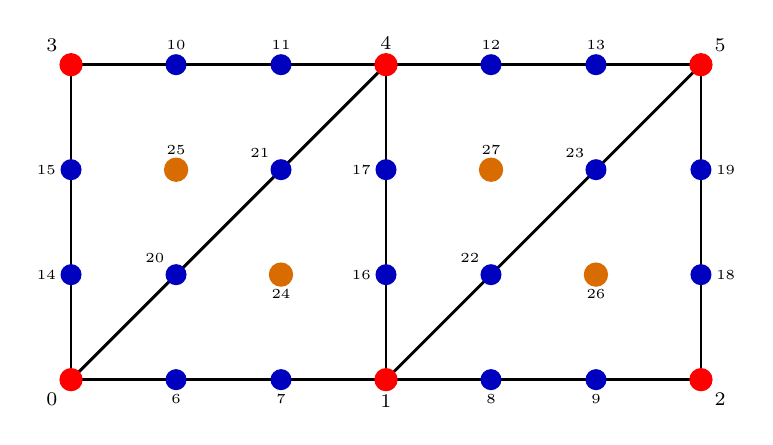
\begin{tikzpicture}[scale=2.0]
  \coordinate (V0) at (0,0);
  \coordinate (V1) at (2,0);
  \coordinate (V2) at (4,0);
  \coordinate (V3) at (0,2);
  \coordinate (V4) at (2,2);
  \coordinate (V5) at (4,2);

  \draw[black,line width=1.05pt]
    (V0)--(V1)--(V2)--(V5)--(V4)--(V3)--cycle;
  \draw[black,line width=1.05pt] (V1)--(V4);
  \draw[black,line width=1.05pt] (V0)--(V4);
  \draw[black,line width=1.05pt] (V1)--(V5);

  % 顶点：0--5
  \foreach \P in {V0,V1,V2,V3,V4,V5}{
    \fill[red] (\P) circle (2.1pt);
  }
  \node[font=\scriptsize,below left=2pt]  at (V0) {$0$};
  \node[font=\scriptsize,below=2pt]       at (V1) {$1$};
  \node[font=\scriptsize,below right=2pt] at (V2) {$2$};
  \node[font=\scriptsize,above left=2pt]  at (V3) {$3$};
  \node[font=\scriptsize,above=2pt]       at (V4) {$4$};
  \node[font=\scriptsize,above right=2pt] at (V5) {$5$};

  % 全局边内点：6--23
  \coordinate (E6)  at ($(V0)!1/3!(V1)$);
  \coordinate (E7)  at ($(V0)!2/3!(V1)$);
  \coordinate (E8)  at ($(V1)!1/3!(V2)$);
  \coordinate (E9)  at ($(V1)!2/3!(V2)$);
  \coordinate (E10) at ($(V3)!1/3!(V4)$);
  \coordinate (E11) at ($(V3)!2/3!(V4)$);
  \coordinate (E12) at ($(V4)!1/3!(V5)$);
  \coordinate (E13) at ($(V4)!2/3!(V5)$);
  \coordinate (E14) at ($(V0)!1/3!(V3)$);
  \coordinate (E15) at ($(V0)!2/3!(V3)$);
  \coordinate (E16) at ($(V1)!1/3!(V4)$);
  \coordinate (E17) at ($(V1)!2/3!(V4)$);
  \coordinate (E18) at ($(V2)!1/3!(V5)$);
  \coordinate (E19) at ($(V2)!2/3!(V5)$);
  \coordinate (E20) at ($(V0)!1/3!(V4)$);
  \coordinate (E21) at ($(V0)!2/3!(V4)$);
  \coordinate (E22) at ($(V1)!1/3!(V5)$);
  \coordinate (E23) at ($(V1)!2/3!(V5)$);
  \foreach \P in {E6,E7,E8,E9,E10,E11,E12,E13,E14,E15,E16,E17,E18,E19,E20,E21,E22,E23}{
    \fill[blue!75!black] (\P) circle (1.9pt);
  }

  \foreach \P/\lab in {E6/6,E7/7,E8/8,E9/9}{
    \node[font=\tiny,below=2pt] at (\P) {$\lab$};
  }
  \foreach \P/\lab in {E10/10,E11/11,E12/12,E13/13}{
    \node[font=\tiny,above=2pt] at (\P) {$\lab$};
  }
  \foreach \P/\lab in {E14/14,E15/15}{
    \node[font=\tiny,left=2pt] at (\P) {$\lab$};
  }
  \foreach \P/\lab in {E16/16,E17/17}{
    \node[font=\tiny,left=2pt] at (\P) {$\lab$};
  }
  \foreach \P/\lab in {E18/18,E19/19}{
    \node[font=\tiny,right=2pt] at (\P) {$\lab$};
  }
  \node[font=\tiny,above left=1pt]  at (E20) {$20$};
  \node[font=\tiny,above left=1pt]  at (E21) {$21$};
  \node[font=\tiny,above left=1pt]  at (E22) {$22$};
  \node[font=\tiny,above left=1pt]  at (E23) {$23$};

  % 单元内部点：24--27
  \coordinate (C24) at (1.333,0.667);
  \coordinate (C25) at (0.667,1.333);
  \coordinate (C26) at (3.333,0.667);
  \coordinate (C27) at (2.667,1.333);
  \foreach \P in {C24,C25,C26,C27}{
    \fill[orange!85!black] (\P) circle (2.2pt);
  }
  \node[font=\tiny,below=2pt] at (C24) {$24$};
  \node[font=\tiny,above=2pt] at (C25) {$25$};
  \node[font=\tiny,below=2pt] at (C26) {$26$};
  \node[font=\tiny,above=2pt] at (C27) {$27$};
\end{tikzpicture}

\end{frame}

\begin{frame}{Hu--Zhang 元的局部自由度编号}
\begin{columns}[c,onlytextwidth]
\column{0.32\textwidth}

二维 $\mathbb P_3$ 情形：

\begin{itemize}
  \item 每个顶点有 $3$ 个分量；
  \item 每个边内格点有 $2$ 个法向分量；
  \item 边按对顶点顺序 $e_0,e_1,e_2$ 编号；
  \item 其余单元局部 bubble 统一排在最后。
\end{itemize}

\[
\dim P_3(K;\mathbb S)=30.
\]

\column{0.66\textwidth}
\centering
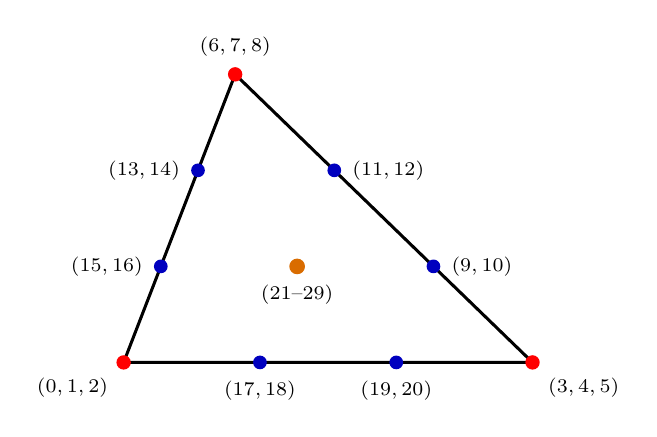
\begin{tikzpicture}[scale=1.18]
  \coordinate (A) at (0,0);
  \coordinate (B) at (4.4,0);
  \coordinate (C) at (1.2,3.1);
  \coordinate (P01) at ($(A)!1/3!(B)$);
  \coordinate (P02) at ($(A)!2/3!(B)$);
  \coordinate (P12) at ($(B)!1/3!(C)$);
  \coordinate (P21) at ($(B)!2/3!(C)$);
  \coordinate (P20) at ($(C)!1/3!(A)$);
  \coordinate (P10) at ($(C)!2/3!(A)$);
  \coordinate (G) at (1.867,1.033);

  \draw[black,line width=1.1pt] (A)--(B)--(C)--cycle;
  \foreach \P in {A,B,C}{\fill[red] (\P) circle (2.2pt);}
  \foreach \P in {P01,P02,P12,P21,P20,P10}{
    \fill[blue!75!black] (\P) circle (2.1pt);
  }
  \fill[orange!85!black] (G) circle (2.4pt);

  \node[font=\scriptsize,below left=3pt]  at (A) {$(0,1,2)$};
  \node[font=\scriptsize,below right=3pt] at (B) {$(3,4,5)$};
  \node[font=\scriptsize,above=3pt]       at (C) {$(6,7,8)$};

  \node[font=\scriptsize,right=3pt] at (P12) {$(9,10)$};
  \node[font=\scriptsize,right=3pt] at (P21) {$(11,12)$};
  \node[font=\scriptsize,left=3pt]  at (P20) {$(13,14)$};
  \node[font=\scriptsize,left=3pt]  at (P10) {$(15,16)$};
  \node[font=\scriptsize,below=3pt] at (P01) {$(17,18)$};
  \node[font=\scriptsize,below=3pt] at (P02) {$(19,20)$};
  \node[font=\scriptsize,below=3pt] at (G) {$(21\text{--}29)$};
\end{tikzpicture}
\end{columns}

\end{frame}

\begin{frame}{Hu--Zhang 元的全局自由度编号}
同样的，全局编号从顶点开始，依次为边内点、单元内部点。

\vspace{5pt}

\centering
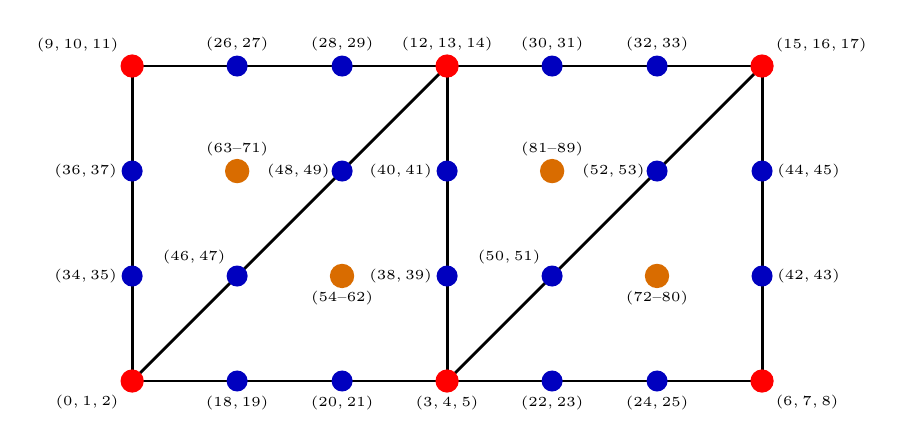
\begin{tikzpicture}[scale=2.0]
  \coordinate (V0) at (0,0);
  \coordinate (V1) at (2,0);
  \coordinate (V2) at (4,0);
  \coordinate (V3) at (0,2);
  \coordinate (V4) at (2,2);
  \coordinate (V5) at (4,2);

  \draw[black,line width=1.05pt]
    (V0)--(V1)--(V2)--(V5)--(V4)--(V3)--cycle;
  \draw[black,line width=1.05pt] (V1)--(V4);
  \draw[black,line width=1.05pt] (V0)--(V4);
  \draw[black,line width=1.05pt] (V1)--(V5);

  % 顶点自由度：0--17
  \foreach \P in {V0,V1,V2,V3,V4,V5}{\fill[red] (\P) circle (2.1pt);}
  \node[font=\tiny,below left=2pt]  at (V0) {$(0,1,2)$};
  \node[font=\tiny,below=2pt]       at (V1) {$(3,4,5)$};
  \node[font=\tiny,below right=2pt] at (V2) {$(6,7,8)$};
  \node[font=\tiny,above left=2pt]  at (V3) {$(9,10,11)$};
  \node[font=\tiny,above=2pt]       at (V4) {$(12,13,14)$};
  \node[font=\tiny,above right=2pt] at (V5) {$(15,16,17)$};

  % 全局边上的法向自由度：18--53
  \coordinate (E18) at ($(V0)!1/3!(V1)$);
  \coordinate (E20) at ($(V0)!2/3!(V1)$);
  \coordinate (E22) at ($(V1)!1/3!(V2)$);
  \coordinate (E24) at ($(V1)!2/3!(V2)$);
  \coordinate (E26) at ($(V3)!1/3!(V4)$);
  \coordinate (E28) at ($(V3)!2/3!(V4)$);
  \coordinate (E30) at ($(V4)!1/3!(V5)$);
  \coordinate (E32) at ($(V4)!2/3!(V5)$);
  \coordinate (E34) at ($(V0)!1/3!(V3)$);
  \coordinate (E36) at ($(V0)!2/3!(V3)$);
  \coordinate (E38) at ($(V1)!1/3!(V4)$);
  \coordinate (E40) at ($(V1)!2/3!(V4)$);
  \coordinate (E42) at ($(V2)!1/3!(V5)$);
  \coordinate (E44) at ($(V2)!2/3!(V5)$);
  \coordinate (E46) at ($(V0)!1/3!(V4)$);
  \coordinate (E48) at ($(V0)!2/3!(V4)$);
  \coordinate (E50) at ($(V1)!1/3!(V5)$);
  \coordinate (E52) at ($(V1)!2/3!(V5)$);
  \foreach \P in {E18,E20,E22,E24,E26,E28,E30,E32,E34,E36,E38,E40,E42,E44,E46,E48,E50,E52}{
    \fill[blue!75!black] (\P) circle (1.9pt);
  }

  \foreach \P/\a/\b in {E18/18/19,E20/20/21,E22/22/23,E24/24/25}{
    \node[font=\tiny,below=2pt] at (\P) {$(\a,\b)$};
  }
  \foreach \P/\a/\b in {E26/26/27,E28/28/29,E30/30/31,E32/32/33}{
    \node[font=\tiny,above=2pt] at (\P) {$(\a,\b)$};
  }
  \foreach \P/\a/\b in {E34/34/35,E36/36/37,E38/38/39,E40/40/41}{
    \node[font=\tiny,left=2pt] at (\P) {$(\a,\b)$};
  }
  \foreach \P/\a/\b in {E42/42/43,E44/44/45}{
    \node[font=\tiny,right=2pt] at (\P) {$(\a,\b)$};
  }
  \node[font=\tiny,above left=1pt] at (E46) {$(46,47)$};
  \node[font=\tiny,left =1pt] at (E48) {$(48,49)$};
  \node[font=\tiny,above left=1pt] at (E50) {$(50,51)$};
  \node[font=\tiny,left =1pt] at (E52) {$(52,53)$};

  % 每个单元的局部 bubble：54--89
  \coordinate (C0) at (1.333,0.667);
  \coordinate (C1) at (0.667,1.333);
  \coordinate (C2) at (3.333,0.667);
  \coordinate (C3) at (2.667,1.333);
  \foreach \P in {C0,C1,C2,C3}{\fill[orange!85!black] (\P) circle (2.2pt);}
  \node[font=\tiny,below=2pt] at (C0) {$(54\text{--}62)$};
  \node[font=\tiny,above=2pt] at (C1) {$(63\text{--}71)$};
  \node[font=\tiny,below=2pt] at (C2) {$(72\text{--}80)$};
  \node[font=\tiny,above=2pt] at (C3) {$(81\text{--}89)$};
\end{tikzpicture}

\end{frame}

\section{矩阵组装}

%------------------------------------------------
\begin{frame}{线弹性问题的混合形式}
\begingroup
\small
\setlength{\abovedisplayskip}{4pt}
\setlength{\belowdisplayskip}{4pt}

考虑线弹性问题：求对称应力张量 $\sigma$ 和位移 $u$，使得
\[
\left\{
\begin{aligned}
\mathcal A\sigma-\varepsilon(u)&=0
&&\text{in }\Omega,\\
-\operatorname{div}\sigma&=f
&&\text{in }\Omega,\\
u&=0
&&\text{on }\partial\Omega,
\end{aligned}
\right.
 \]

其中，$\mathcal A$ 是柔度算子；$\varepsilon(u)$ 是位移的对称梯度：
\[
\mathcal{A} \sigma =
\frac{1}{2\mu}\left(\sigma-\frac{\lambda}{d\lambda+2\mu}
\operatorname{tr}(\sigma)I\right),\quad 
\varepsilon(u)
=
\frac12\bigl(\nabla u+\nabla u^{T}\bigr),
\quad
\sigma(x)\in\mathbb S.
\]

取应力空间和位移空间
\[
\Sigma=H(\operatorname{div};\Omega;\mathbb S),
\qquad
V=L^2(\Omega;\mathbb R^d).
\]

Hellinger--Reissner 混合形式为：求
$(\sigma,u)\in\Sigma\times V$，使得
\[
\begin{aligned}
(\mathcal A\sigma,\tau)
+(\operatorname{div}\tau,u)
&=0,
&&\forall\tau\in\Sigma,\\
(\operatorname{div}\sigma,v)
&=-(f,v),
&&\forall v\in V.
\end{aligned}
\]

Hu--Zhang 离散空间取为
$\Sigma_h=\Sigma_{h,k}^{\mathrm{HZ}}$，
$V_h=\mathbb P_{k-1}(\mathcal T_h;\mathbb R^d)$。
\endgroup
\end{frame}


%------------------------------------------------
\begin{frame}{离散系统的矩阵形式}

取全局基函数
$$
\Sigma_h=\operatorname{span}\{\Phi_i\}_{i=1}^{N_\sigma},
\qquad
V_h=\operatorname{span}\{\psi_r\}_{r=1}^{N_u},
$$
设数值解 $\sigma_h \in\Sigma_h$ 和 $u_h\in V_h$ 为
$$
\sigma_h=\sum_{j=1}^{N_\sigma}\sigma_j\Phi_j,
\qquad
u_h=\sum_{s=1}^{N_u}u_s\psi_s.
$$

定义矩阵
$$
M_{ij}
=
\sum_{K\in\mathcal T_h}
\int_K
\mathcal A\Phi_j:\Phi_i\,dx,
\qquad
B_{ri}
=
\sum_{K\in\mathcal T_h}
\int_K
\operatorname{div}\Phi_i\cdot\psi_r\,dx,
\qquad
F_r
=
\sum_{K\in\mathcal T_h}
\int_K f\cdot\psi_r\,dx.
$$

离散系统为
$$
\begin{bmatrix}
M&B^T\\
B&0
\end{bmatrix}
\begin{bmatrix}
\boldsymbol{\sigma}\\
\boldsymbol{u}
\end{bmatrix}
=
\begin{bmatrix}
0\\
-\boldsymbol{F}
\end{bmatrix}.
$$

\end{frame}


%------------------------------------------------
\begin{frame}{逐单元计算与全局组装}

设单元 $K$ 上的局部基函数分别为
$$
\{\Phi_i^K\}_{i=1}^{n_\sigma},
\qquad
\{\psi_r^K\}_{r=1}^{n_u}.
$$

局部矩阵和右端项为
$$
(M_K)_{ij}
=
\int_K
\mathcal A\Phi_j^K:\Phi_i^K\,dx,
$$
$$
(B_K)_{ri}
=
\int_K
\operatorname{div}\Phi_i^K\cdot\psi_r^K\,dx,
\qquad
(F_K)_r
=
\int_K f\cdot\psi_r^K\,dx.
$$

设 $R_K^\sigma$ 和 $R_K^u$ 为局部到全局的自由度映射，则
$$
M
=
\sum_{K\in\mathcal T_h}
(R_K^\sigma)^T M_KR_K^\sigma,
$$
$$
B
=
\sum_{K\in\mathcal T_h}
(R_K^u)^TB_KR_K^\sigma,
\qquad
F
=
\sum_{K\in\mathcal T_h}
(R_K^u)^TF_K.
$$

\end{frame}


%------------------------------------------------
\begin{frame}{单纯形上的数值积分}
\begingroup
\small
\setlength{\abovedisplayskip}{4pt}
\setlength{\belowdisplayskip}{4pt}

在单元 $K$ 上取重心坐标积分公式
$\{( x_q, w_q)\}_{q=1}^{N_q},$ 
因此
\[
\int_K g(x)\,dx
\approx
|K|
\sum_{q=1}^{N_q}
 w_q
g\bigl(x_q\bigr).
\]

三个局部量可在同一组积分点上计算：
\[
\begin{aligned}
(M_K)_{ij}
&\approx
|K|\sum_{q=1}^{N_q} w_q\,
\mathcal A\Phi_j^K(x_q):\Phi_i^K(x_q),\\
(B_K)_{ri}
&\approx
|K|\sum_{q=1}^{N_q} w_q\,
\operatorname{div}\Phi_i^K(x_q)\cdot\psi_r^K(x_q),\\
(F_K)_r
&\approx
|K|\sum_{q=1}^{N_q} w_q\,
f(x_q)\cdot\psi_r^K(x_q).
\end{aligned}
\]

\endgroup
\end{frame}

\section{程序实现}
\begin{frame}{框架设计}

整体程序可以分成四层：
$$
\texttt{Mesh}
\quad\longrightarrow\quad
\texttt{FiniteElementSpace}
\quad\longrightarrow\quad
\texttt{Assembler}
\quad\longrightarrow\quad
\texttt{Solver}.
$$

\vspace{0.5em}

\begin{itemize}
  \item \texttt{Mesh}：保存网格几何与拓扑关系；
  \item \texttt{FiniteElementSpace}：生成自由度编号、基函数和局部映射；
  \item \texttt{Assembler}：计算局部矩阵并组装全局系统；
  \item \texttt{Solver}：处理线性系统、预条件和后处理。
\end{itemize}

\vspace{0.5em}

Hu--Zhang 元的重点在第二层：
$$
\texttt{basis evaluation}
+
\texttt{dof map}
+
\texttt{normal continuity}.
$$

\end{frame}

\begin{frame}{网格模块}

输入：
$$
\texttt{node},
\qquad
\texttt{cell}.
$$

输出派生数据：
$$
\texttt{edge},\quad
\texttt{face},\quad
\texttt{cell2edge},\quad
\texttt{cell2face},
$$
$$
\texttt{edge2cell},\quad
\texttt{face2cell},\quad
\texttt{bdFlag},\quad
\texttt{orientation}.
$$

\vspace{0.4em}

主要函数：
\begin{itemize}
  \item 构造全局边、面编号；
  \item 计算单元体积、Jacobian、重心坐标梯度；
  \item 判断边界边、边界面；
  \item 记录局部方向与全局方向的关系。
\end{itemize}

\end{frame}

\begin{frame}{空间模块}

空间模块负责从网格生成有限元空间。

\vspace{0.4em}

\begin{itemize}
  \item Lagrange 空间：生成等距格点与标量基函数；
  \item Hu--Zhang 空间：生成矩阵值方向与局部基函数；
  \item 自由度编号：构造 \texttt{elem2dof}；
  \item 基函数评价：计算 $\Phi_i$ 与 $\operatorname{div}\Phi_i$；
  \item 方向修正：处理边方向、面方向和法向符号。
\end{itemize}

\vspace{0.5em}

核心数据：
$$
\texttt{localDof},
\qquad
\texttt{globalDof},
\qquad
\texttt{elem2dof},
\qquad
\texttt{basisValue}.
$$

\end{frame}

\begin{frame}{算法模块}

算法模块围绕局部矩阵和全局系统展开。

\vspace{0.4em}

\begin{itemize}
  \item \texttt{LocalMass}：计算应力质量矩阵 $M_K$；
  \item \texttt{LocalDiv}：计算散度耦合矩阵 $B_K$；
  \item \texttt{Assemble}：根据 \texttt{elem2dof} 组装全局矩阵；
  \item \texttt{Condense}：局部消去 bubble 自由度；
  \item \texttt{Solve}：直接法或迭代法求解；
  \item \texttt{PostProcess}：误差、残量和可视化输出。
\end{itemize}

\vspace{0.4em}

高阶实现中可以进一步加入
$$
\texttt{reference precompute},
\qquad
\texttt{matrix-free LocalApply}.
$$

\end{frame}

\begin{frame}{相关库}

\begin{itemize}
  \item \textbf{线性代数：}Eigen，BLAS/LAPACK；
  \item \textbf{稀疏直接法：}MUMPS，PARDISO；
  \item \textbf{迭代法与预条件：}AMG，Hypre，PETSc；
  \item \textbf{网格与划分：}Gmsh，METIS，ParMETIS；
  \item \textbf{并行：}OpenMP，MPI；
  \item \textbf{可视化：}VTK，ParaView。
\end{itemize}

\vspace{0.6em}

本报告中的实现重点：
$$
\text{网格拓扑}
\quad+
\text{自由度编号}
\quad+
\text{Hu--Zhang 局部基函数}
\quad+
\text{矩阵组装}.
$$

\end{frame}

\end{document}
